%%%%%%%%%%%%%%%%%%%%%%%%%%%%%%%%%%%%%%%%%%%%%%%%%%%%%%%%%%%%%%%%%%%%%
%%%
%%% Set these variables appropriately
%%%
\newcommand{\AUTHORS}{Qizhe Cai \quad Wei Hu \quad Yueyang Qiu \\ \{qizhec,huwei,yqiu\}@cs.princeton.edu}
\newcommand{\TITLE}{COS 561 Final Project: AccWeb -- Improving Web Performance via Prefetching}
\newcommand{\KEYWORDS}{}
\newcommand{\CONFERENCE}{}
\newcommand{\PAGENUMBERS}{yes}       % "yes" or "no"
\newcommand{\TOAPPEAR}{no}
%%%
%%%
%%%%%%%%%%%%%%%%%%%%%%%%%%%%%%%%%%%%%%%%%%%%%%%%%%%%%%%%%%%%%%%%%%%%%

%%%% Setup the document/page
\documentclass[pdftex,twoside,twocolumn,11pt,letterpaper]{article}
\usepackage{ifthen}
\usepackage{amsmath}
\usepackage{chngcntr}

\ifthenelse{\equal{\PAGENUMBERS}{yes}}{%
\usepackage[nohead,
            left=1in,right=1in,top=1in,
            footskip=0.5in,bottom=0.75in     % Room for page numbers
            ]{geometry}
}{%
\usepackage[noheadfoot,columnsep=0.2in,
            margin=1in,centering,truedimen]{geometry}
}

\usepackage{fancyhdr}
\usepackage[numbers,sort]{natbib}
\usepackage{xspace}
\usepackage{booktabs}
\usepackage{subfigure}
\usepackage[T1]{fontenc}
\usepackage{textcomp}
\usepackage{mathptmx}   % Times + Times-like math symbols
\usepackage{courier}
\usepackage[scaled=0.92]{helvet}

\usepackage{color}
\usepackage[pdftex]{graphicx}
\ifthenelse{\isundefined{\wantBW}}{%
  \usepackage[colorlinks]{hyperref}%        % for online version
}{%
  \usepackage[pdfborder={0 0 0}]{hyperref}% % for paper (B&W) version
}
\newcommand{\URL}[1]{\url{#1}}

%%%%% Setup for PDF
\hypersetup{%
pdfauthor = {\AUTHORS},
pdftitle = {\TITLE},
pdfsubject = {\CONFERENCE},
pdfkeywords = {\KEYWORDS},
bookmarksopen = {true}
}

%\setlength{\parindent}{0pt}
%\setlength{\parskip}{0pt}
\renewcommand{\headrulewidth}{0pt}
\newcommand{\Paragraph}[1]{\vspace{-2ex}\paragraph{#1.}}
\setlength{\topmargin}{-.15in}

\ifthenelse{\equal{\PAGENUMBERS}{yes}}{%
  \pagestyle{plain}
}{%
  \pagestyle{empty}
}

\makeatletter\long\def\@makecaption#1#2{
   \vskip 10pt
   \setbox\@tempboxa\hbox{\textsf{#1: #2}}
   \ifdim \wd\@tempboxa >\hsize % IF longer than one line:
       \textsf{#1: #2}\par      % THEN set as ordinary paragraph.
     \else                      % ELSE  center.
       \hbox to\hsize{\hfil\box\@tempboxa\hfil}
   \fi}
\makeatother

\clubpenalty=10000  % Don't allow orphans
\widowpenalty=10000 % Don't allow widows

\title{\textbf{\TITLE}}
\author{\AUTHORS}
\date{}

% Compact itemize and enumerate.  Note that they use the same counters and
% symbols as the usual itemize and enumerate environments.
\def\compactify{\itemsep=0pt \topsep=0pt \partopsep=0pt \parsep=0pt}
\let\latexusecounter=\usecounter
\newenvironment{CompactItemize}
  {\def\usecounter{\compactify\latexusecounter}
   \begin{itemize}}
  {\end{itemize}\let\usecounter=\latexusecounter}
\newenvironment{CompactEnumerate}
  {\def\usecounter{\compactify\latexusecounter}
   \begin{enumerate}}
  {\end{enumerate}\let\usecounter=\latexusecounter}

\newcommand{\comment}[1]{\textcolor{red}{#1}}
\newcommand{\ignore}[1]{}

\newcommand{\xc}[1]{\mbox{\textit{#1}}}
\newcommand{\la}{\leftarrow}
\newcommand{\ra}{\rightarrow}
\newcommand{\somespace}{\hspace{0.1cm}}

\def\discretionaryslash{\discretionary{/}{}{/}}
\def\discretionarydot{\discretionary{.}{}{.}}
\def\discretionarycolon{\discretionary{:}{}{:}}
{\catcode`\/\active
\catcode`\.\active
\catcode`\:\active
\gdef\URLprepare{\catcode`\/\active\let/\discretionaryslash
                 \catcode`\.\active\let.\discretionarydot
                 \catcode`\:\active\let:\discretionarycolon
        \def~{\char`\~}}}%
\def\URL{\bgroup\URLprepare\realURL}%
\def\realURL#1{\tt #1\egroup}%

\newcommand{\eg}{{\em e.g.}, }
\newcommand{\ie}{{\em i.e.}, }
\newcommand{\etal}{{\em et al.\ }}

\def\check{\stackrel{{\scriptscriptstyle ?}}{=}}




\begin{document}
\maketitle

% -*-LaTeX-*-
% $Id: abstract.tex 70 2007-01-30 21:59:16Z nicolosi $

\begin{abstract}
We present AccWeb (Accelerated Web), a web service that improves user experience of web browsing. AccWeb improves web performance by prefetching web resources when the user is typing in the address bar. In order to prefetch resources, AccWeb predicts the URL that the user wants to navigate. The prediction is based on the user's browsing history and typing behaviors. After a prediction is made, all demanded resources belonging to the predicted URL will be prefetched. Also, AccWeb gives users options to choose types of resources to prefetch -- users can select the types of resources to prefetch based on their own preferences as well as real-time network condition. We build an AccWeb prototype, and our experiments show that the performance of browsers installing AccWeb is much better than the performance of browsers without AccWeb.
\end{abstract}

   
\section{Introduction}
\label{sec:intro}

Despite the prevalence of internet accesses on PCs and mobile devices, many users are complaining about their experiences of poor web performances. Current approaches to improving web performance mainly focus on designing new protocols (e.g. SPDY, HTTP/2) which make communication between servers and clients more efficient. For example, HTTP/2 reduces loading times by multiplexing multiple requests over a single TCP connection. However, with all these advancements, page loading times are still likely to exceed user tolerance limits for the foreseeable future, due to user expectations on lower loading times and richer web contents. In this project, instead of trying to further improve the speed of communications between servers and clients, we are interested in developing a user-oriented web service in order to speed up page loading time. In particular, we focus on the technique of prefetching web contents while the user is typing in the address bar.

Prefetching a web resource only makes sense when the resource is \emph{static}, i.e., its URL pattern keeps unchanged for a long period of time. In order to evaluate whether prefetching is useful or not, we estimate the percentage of static web resources by testing the top 20 news websites on Alexa. Our result shows that around 70\% of resources are static (see Fig.~\ref{fig:static_resource_precentage}). Therefore, prefetching static web resources can indeed improve web performance. Moreover, the bandwidth and the number of TCP connections per domain of a browser for loading web resources are limited. If the static resources are prefetched, non-static resources can be loaded faster without the competitions from static ones.

\begin{figure}[htbp] 
	\centering
	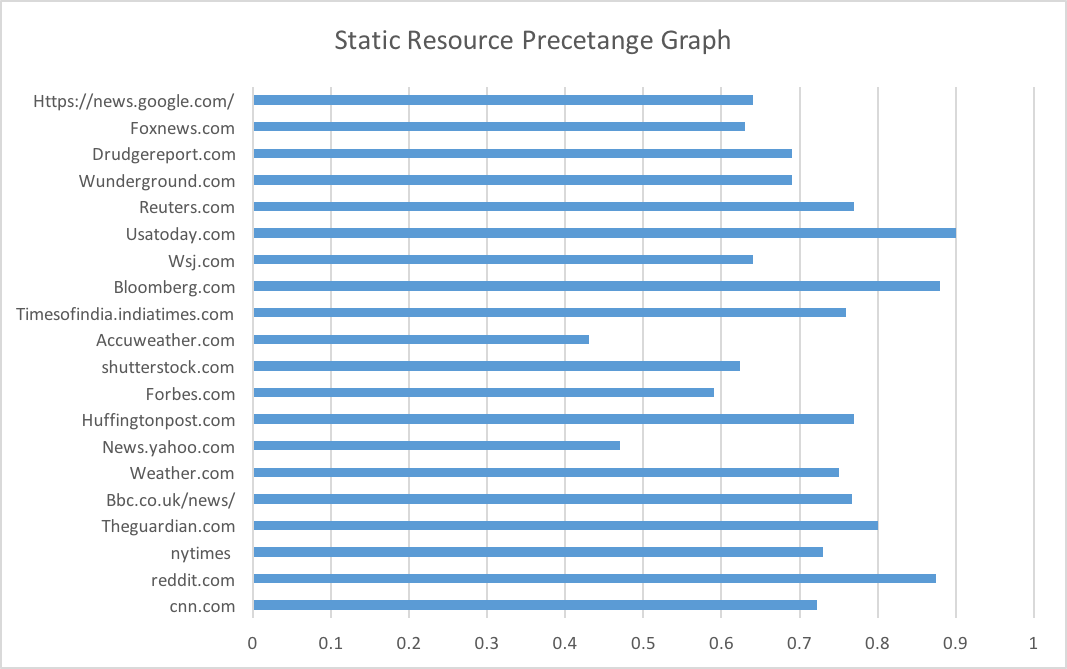
\includegraphics[width=0.5\textwidth]{static_resource_precentage.png}  
	\caption{Percentages of static resources in Alexa's top 20 news websites.}
	\label{fig:static_resource_precentage}
\end{figure} 

In fact, some browsers such as Chrome already have built-in prefetching services based on URL prediction. However, we find that Chrome's prefetching mechanism falls short in the following aspects:
\begin{itemize}
	\item URL Prediction is based on the user's browsing history. If the user clears browsing data, then prediction cannot happen, which means no web resources can be preloaded.
	\item The set of URLs eligible to be prefetched is too conservative, compared with the URLs that the user has typed in the address bar before. Only a small number of websites that are visited most frequently can be prefetched by Chrome.
	\item When a URL is predicted, the majority of the web resources associated with that URL will be preloaded, regardless of the user's need. For that reason, the cost of prefetching unneeded web resources will be huge if Chrome predicts the URL incorrectly, especially when the network bandwidth is limited.
\end{itemize}

We develop AccWeb, a prefetching service with good performance while dealing with the above drawbacks of Chrome. AccWeb runs in 3 separate stages.
\begin{enumerate}
	\item Analyzing. In this stage, AccWeb fetches and records all static web resources of URLs that the user has already visited in the past.
	\item Predicting. Based on the user's typing and browsing history, AccWeb predicts the URL that the user currently tries to navigate (if the prediction confidence is high enough) given the user's current input in the address bar.
	\item Prefetching. After receiving the predicted webpage, The URLs of the web resources on that page are sent through the HTTP link header field to the browser, and the browser starts to preload these resources.
\end{enumerate}
%The second stage is predicting. Based on the user's typing and browsing history, AccWeb predicts the URL that the user currently tries to navigate (if the prediction confidence is high enough) given the user's current input in the address bar.
%The third stage is prefetching. After receiving the predicted webpage, The URLs of the web resources on that page are sent through the HTTP link header field to the browser, and the browser starts to preload these resources.
The demo of AccWeb can be found at \href{https://github.com/caiqizhe/COS561_final_project}{this link}.

AccWeb eliminates (or at least alleviates) the abovementioned drawbacks of Chrome. First, the user's browsing history is stored in a browser extension called Predictor, so flushing browser history in the browser does not affect prefetching in AccWeb. Second, we design a prediction mechanism that is less conservative than Chrome's, while ensuring a high confidence level. Third, we allow the users to have control over which kinds of resources to be prefetched. Note that different users may have different preferences regarding web performance: some users like to load images as quickly as possible, while others care more about the loading time of texts. In addition, under poor network condition, users might want to limit the prefetching service to lower the cost of wrong predictions and to save bandwidth. We implement different modes (e.g. full mode, limited mode, image mode, etc.) that users can select based on their preferences and network condition.



\section{Design}
\label{sec:design}

In this section, we describe the design of AccWeb. The architecture and the workflow of AccWeb is shown in Fig.~\ref{fig:arch}. It is divided into three stages by their functional purposes: analyzing, predicting, and prefetching.

\begin{figure}[htbp] 
	\centering
	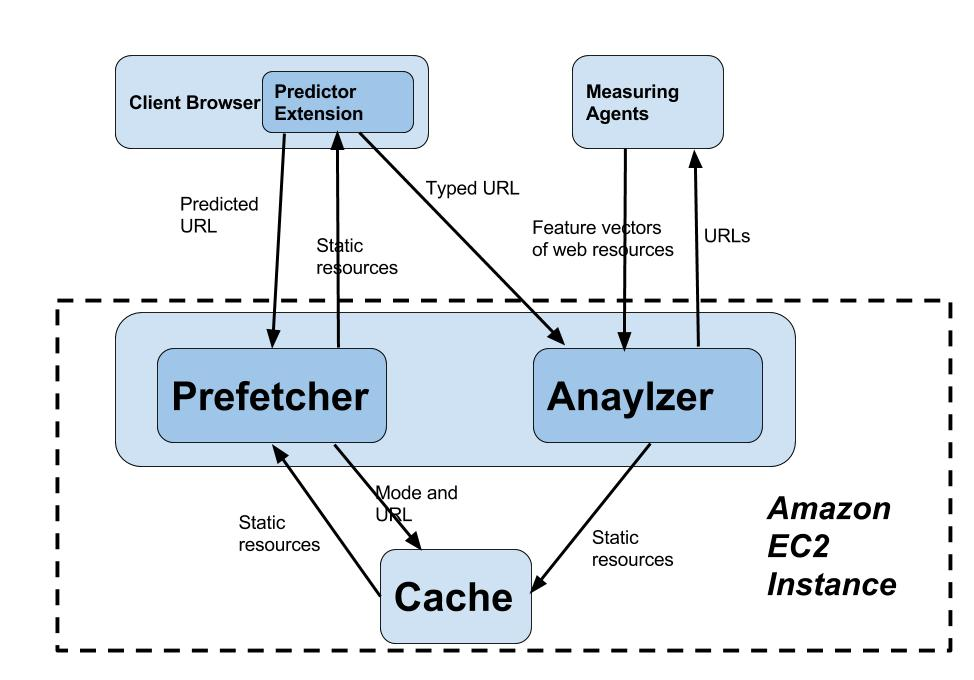
\includegraphics[width=0.5\textwidth]{ACCWeb-Arch-3.jpg}  
	\caption{AccWeb architecture.}
	\label{fig:arch}
\end{figure} 

\subsection{Analyzing}

Analyzer is a Python server running on Amazon EC2 instance. Analyzer gets all URLs the user has visited and then sends these URLs to Measuring Agents. Measuring Agents navigate these websites, record all feature vectors of web resources, and send them back to Analyzer. A feature vector includes the type of resources, the time of sending requests, the time of getting responses, and so on. After analyzing data (which will be explained in Section~\ref{sec:details}), Analyzer forms potential responses for prefetching, and stores them in the cache.

\subsection{Predicting}

Predictor is a Chrome extension running on client browser and is responsible for predicting. Predictor records the user's typed texts and navigated URLs, and builds a prediction table. Utilizing this table, we design an algorithm to predict the URL the user wants to navigate based on his/her current input in the address bar. Since Predictor stores all the data in the extension itself, when the user flushes the browsing history, it still can predict URL the user wants to navigate. Also, unlike Chrome, the set of URLs that will be prefetched in AccWeb is almost the same as the browsing history of the user, which allows much more flexibility. After Predictor sends the predicted URL to Prefetcher, Prefetcher will send back all resources that will be loaded. Details of our prediction algorithm will be explained in Section~\ref{sec:details}.

\subsection{Prefetching}

Prefetcher is a Python server running on Amazon EC2 instance. Depending on real-time network condition and the user's own preference, the user can select his/her favorite prefetching mode in the Chrome extension. The available modes are full mode, limit mode, image mode, script mode and DNS-prefetch mode. The details of these modes will be explained in Section~\ref{sec:details}. After receiving the predicted URL and the current mode from the extension, Prefetcher fetches corresponding resources from cache and sends them back to the extension.

%As discussed, Chrome users currently have no choice to select which types of resources to preload. Since Chrome prefetches all static resources, the cost of misprediction is very high, especially if the network is on congestion. Using AccWeb, the user can choose the mode that meets his/her need as well as the network condition. On poor network condition, users may select limit mode or even DNS-prefetch mode to reduce the bandwidth of prefetching. Also, different users may have different preferences. The image mode and the script mode cater to these preferences.
\section{Implementation Details}
\label{sec:details}

In this section, we present the implementation details of the three components of AccWeb.

\subsection{Analyzing}

There are three steps in Analyzer. First, Analyzer gets all static web resources, including the domain names for DNS prefetching and HTTP web requests for preloading. Second, Analyzer filters out those static web requests that the the browser does not need to prefetch. Third, Analyzer forms link headers for each mode and stores headers in the cache.

In the first step, Analyzer gets all HTTP static requests. Measuring Agents navigate the same URL multiple times, and send back to Analyzer feature vectors of all HTTP web requests. A feature vector contains information like type of web resource, time of sending requests, and time of getting responses. These features will be used in different prefetching modes. For example, in the script mode, only resources with the script type are prefetched. By checking the recurrence of web requests, Analyzer fetches all static HTTP web requests. Besides HTTP web requests, domain names are static resources as well, which can be used for DNS-prefetch.

Second, not all static HTTP requests need to be prefetched. Web developers set some web resources' expire date the same date as or even earlier than the current date in HTTP headers. 
These web resources must be fetched every time when the browser loads webpages, even if resources have already been in the cache. In this case, Analyzer discards these resources from the cache. This step can prevent unnecessary prefetching, which is particularly important for the limit mode. (In the limit mode, AccWeb only selects six HTTP web requests to prefetch per domain.) %If some web resources become expired immediately after prefetched, the limit mode will be ineffective since there are few prefetched resources that can be used during loading a web page.

After storing all static web resources in the cache, Analyzer forms link HTTP headers for different modes and stores headers to cache as well. This step can save the time of forming headers when the browser preloads static resources in a web page. When Predictor sends predicted URL to Prefetcher, Prefetcher gets responses directly from cache rather than spends extra time on forming link headers. Reducing the total time of fetching static resources improves the web performance of loading websites.  

\subsection{Prediction}

The goal of Predictor is to accurately predict the URL that the user wants to visit based on his/her current input in the address bar. We first build a prediction table to store the user's typing and browsing history, which can be updated when there is a new browsing record, and then use this table to make predictions.

Each entry in the prediction table records the user's browsing information about a (string, URL) pair. For every such pair in the table, we store 3 attributes: hit count, miss count, and confidence. We construct the table as follows. If the user types the string \textsf{str1} in the address bar and visits the URL \textsf{url1}, then for all prefix \textsf{pfx} of \textsf{str1}:
\begin{itemize}
	\item The hit count of (\textsf{pfx}, \textsf{url1}) will increase by $1$. If the pair (\textsf{pfx}, \textsf{url1}) is not in the table, it will be added to the table with hit count $1$ and miss count $0$.
	\item For any other URL \textsf{url2} such that (\textsf{pfx}, \textsf{url2}) is in the table, the miss count of (\textsf{pfx}, \textsf{url2}) will increase by $1$.
\end{itemize}
For each pair, the confidence is defined to be $\frac{\text{hit count}}{\text{hit count} + \text{miss count}}$.

Our rule of prediction is: when the user types a string \textsf{str} in the address bar, find the URL \textsf{url} that maximizes the confidence of (\textsf{str}, \textsf{url}) in the table. Additionally, this pair (\textsf{str}, \textsf{url}) has to satisfy two conditions: (i) the confidence is sufficiently large (say, at least $0.9$); (ii) the hit count is not too small (say, at least $5$).
When making a prediction for prefetching, we really want the prediction to be correct otherwise the prefetching will be a waste of resources, so we impose these two restrictions. If either of these conditions is not satisfied, we will not make any prediction.

We also propose a variant that extends the above prediction method. By the end of every day, we multiply all the hit counts and miss counts in the table by a factor less than 1 (say, 0.9). This method explicitly attaches more importance to more recent browsing activities, which makes sense since the user's interests and browsing habits might change over time.



\subsection{Prefetching}

All prefetching actions are done through adding a link header field in the response to Predictor. The link header field is an HTTP header that allows the server to point an interested client to another resource containing metadata about the requested resource. The basic format of a link header is: \[\texttt{Link: <meta.rdf>; rel=meta,}\]
The string between \texttt{<} and \texttt{>} indicates the address of the web resource, and the value of \texttt{rel} specifies the relationship of the web resource to clients or the actions that the browser should do immediately or in the future. Available actions related to prefetching include \texttt{dns-prefetch}, \texttt{preconnect}, \texttt{prefetch}, \texttt{preload} and \texttt{prerender}. In AccWeb, we only use \texttt{dns-prefetch} and \texttt{preload}. After the browser sends an HTTP request to a server, by adding link header field in the HTTP response header, the server can require the browser to get IP address of server (\texttt{dns-prefetch}), set up a TCP connection (\texttt{preconnect}), and load web resources (\texttt{prefetch} or \texttt{preload}).

Compared with sending requests directly by extensions on client browsers, retrieving web resources through link header field has several advantages. First, it is more convenient. The browser extension does not have to send requests directly. Second, types of web resources that can be prefetched are more flexible. The Chrome extension can only send HTTP requests and HTTP responses. Using link headers, AccWeb can ask the browser to send DNS queries, pre-establish TCP connections and send HTTP requests. This can give users more options to prefetch web resources. Third, requests are actually formed and sent by browsers when using link header fields. If web resources are in the cache of browsers, requests will not be formed. If a Chrome extension sends a web request, the browser will first check whether the cache of the browser contains the web resource and then will decide whether it should send the request to servers. This process may take about 10 milliseconds. Although the time is very short, we want to save as much time as possible.

In the following we discuss the different prefetching modes in AccWeb.

\subsubsection*{DNS-prefetch mode}
In the DNS-prefetch mode, AccWeb only prefetches IP addresses of domain names. This mode can be used when the network is in congestion. Prefetching IP addresses does not occupy much bandwidth, while AccWeb can help clients avoid DNS lookup time. The DNS-prefetch format of link header is: 
\begin{align*}
\texttt{Link: ``<'' + hostname + ``>;}\\
\texttt{rel=dns-prefetch,''}
\end{align*}

%\texttt{Link: ``<'' + hostname + ``>; rel=dns-prefetch,''}


\subsubsection*{Full load mode}
In the full load mode, AccWeb prefetches all static resources. This mode can be used when the network condition is pretty good and the user wants to load all the resources quickly. The link header looks like:
\[\texttt{Link: ``<'' + url + ``>; rel=preload,''}\]
This link header is also used in all the modes to be introduced below.


\subsubsection*{Limit mode}
In order to reduce the cost of misprediction, save the bandwidth while still improve the web performance, we design a limit mode. In this mode, AccWeb prefetches only six HTTP web requests per domain. Prefetched HTTP requests are selected randomly. Also, Prefetching six resources per domain reduces the stalled time of web requests when loading webpages. Chrome only allows six TCP connections per domain in the HTTP/1.1 protocol, and the requests that cannot be fetched immediately are stalled in a queue. As some websites have more than thirty web requests in the same domain, the stalled time of web requests may be very long. 

\subsubsection*{Image mode \& script mode}
The image mode and the script mode are for users who mainly concern about the loading time of image or script resources. Using these modes can also save the bandwidth for loading other types of resources.

\section{Evaluation}
\label{sec:eval}

We perform some preliminary experiments to evaluate the effectiveness of AccWeb.

\subsection{Evaluation setup}

Our experiments are conducted using Chrome browser on a Macbook Pro laptop, running macOS Sierra, as the client. This client connects to a WiFi hotspot exported by a TP-LINK router. For simplicity, the client is both measuring agents for analyzing web resources and the user for browsing web pages. We load the full version of web pages using Google Chrome Version 55.0.2883.95 (64-bit) for Mac. We host Prefetcher and Analyzer in a small instance VM in Amazon EC2's US West Region. Predictor is a Google Chrome extension running on the browser of the client. Different experiments have small changes on the setup, which will be explained in the subsections below.


\subsection{Page Loading Time}

We evaluate the improvement in page loading times enabled by the full mode and the limit mode of AccWeb, compared with the loading times without AccWeb. We have two assumptions: first, we assume that our prediction is correct; second, we assume that before the user loads a web page, all static resources required to be prefetched are already loaded - when the browser starts to load web pages, the prefetched resources can be obtained from the cache. We select 50 websites from Alexa's top 150 websites in China, load 10 times for each web page, and record loading time of web pages for the full load mode, the limit mode, and non-prefetching mode. When testing non-prefetching mode, we disable Chrome's default prefetching service.


We plot the CDFs (across websites) of average loading times (Fig.~\ref{fig:average}) and CDFs of median loading times (Fig.~\ref{fig:median}) of the websites in the 3 different modes. As we can see from the plots, there are improvements in loading times when using AccWeb. For example, in the full mode, around 75\% of web pages' average loading times are less than or equal to 2 seconds, while in the non-prefetching mode this fraction is 64\%. This improvement is also evident in median loading times.

\begin{figure}[htbp] 
	\centering
	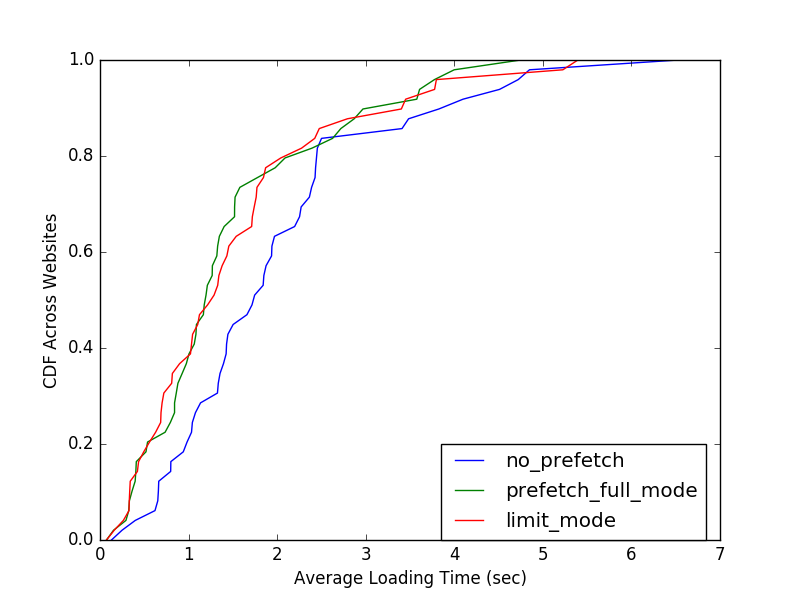
\includegraphics[width=0.5\textwidth]{average.png}  
	\caption{CDFs of average loading times of 50 websites in full mode, limit mode, and non-prefetching mode.}
	\label{fig:average}
\end{figure} 

\begin{figure}[htbp] 
	\centering
	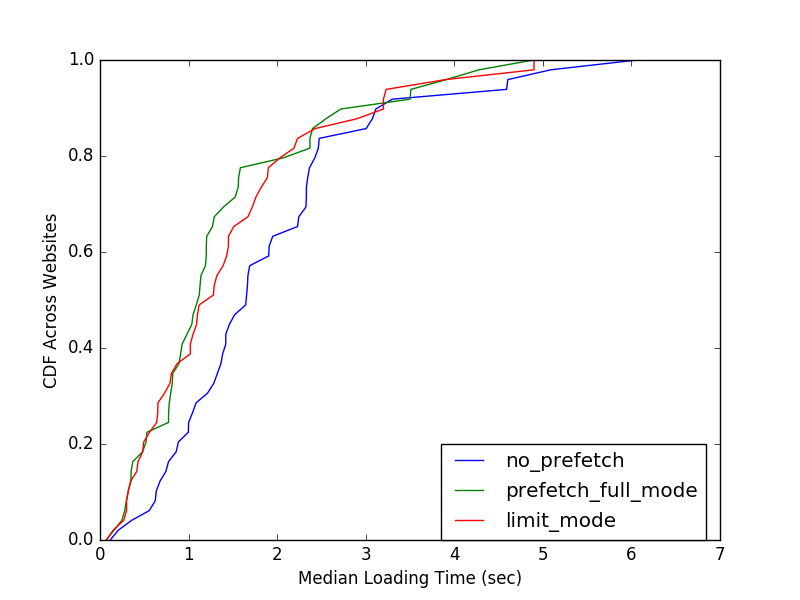
\includegraphics[width=0.5\textwidth]{median.png}  
	\caption{CDFs of median loading times of 50 websites in full mode, limit mode, and non-prefetching mode.}
	\label{fig:median}
\end{figure} 

\subsection{Number of HTTP Reqeusts Prefetched}


We use the same 50 websites from the last experiment to test the number of HTTP requests prefetched in the full mode and the limit mode. For each website, we record the numbers of web requests that are prefetched in both modes. The resulting CDFs are plotted in Fig.~\ref{fig:number_requests}. We can see that the number of requests prefetched in the full mode significantly exceeds the number of requests in the limit mode. In the limit mode, the maximum number of web requests is less than 125. For about 80\% of websites, the number of web requests prefetched in the limit mode is less than 50; in the full mode, this fraction is only 40\%.

Our finding implies that the cost of mispredictions in the full mode can be much higher than the cost in the limit mode. While the loading times in the limit mode shown in Fig.~\ref{fig:average} and Fig.~\ref{fig:median} are not significantly less than the times in the full mode, the difference in misprediction costs can be vital. Hence, when the network bandwidth is limited, we suggest using the limit mode instead of the full mode.


\begin{figure}[htbp] 
	\centering
	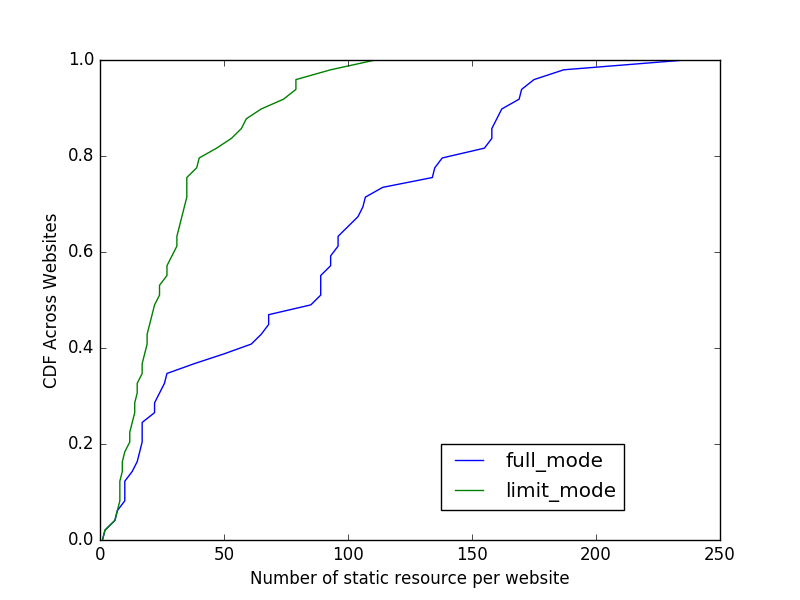
\includegraphics[width=0.5\textwidth]{static_resource.png}  
	\caption{CDFs of the numers of prefetched resources of 50 websites in full mode and limit mode.}
	\label{fig:number_requests}
\end{figure} 












\section{Related Work}
\label{sec:related}

Prefetching contents~\cite{padmanabhan1996using, jiang1998web} and predicting what contents should be prefetched~\cite{palpanas1998web, nanopoulos2003data, chen2003popularity} were previous studied. However, they did not consider overheads of misprediction or limited bandwidth in real time. Some approaches (e.g.~\cite{fan1999web}) utilizes proxies to maximize low-bandwidth users' utility. One problem is that if proxies are down, users cannot connect to the internet.

\section{Conclusion and Future Work}
\label{sec:conclusion}

We develop AccWeb, a web service that performs prefetching to improve user experience of web browsing. AccWeb has a mechanism to predict the URL the user wants to visit when he/she is typing in the browser's address bar, and prefetches the static resources associated with this URL. The user is allowed to select the types of resources to prefetch based on personal preference and network condition. Preliminary experimental results show the effectiveness of AccWeb in reducing page loading times.


There are several directions for further investigation, which we are unable to study due to time limitation.
First, it would be great if AccWeb can adjust to network condition automatically, so that it will switch to limit mode or suggest the user to do so when the network bandwidth is limited.
Second, designing an accurate prediction algorithm that works for different types of users is an interesting problem even in its own. One might borrow ideas from machine learning, and take into consideration many kinds of user behaviors in the prediction process.
Third, how to store the data (user browsing history, potential URLs to be prefetched, etc.) efficiently is a problem worth being studied.



%% Bibliography
%\vspace{-1ex}
%\linespread{1.0}
%\setlength{\bibsep}{1pt}
%\footnotesize
\small
\bibliography{local}
\bibliographystyle{abbrvnat}

\end{document}

